% !TEX root = mainPart.tex
\documentclass[12pt]{book}
\usepackage[utf8]{inputenc}

%% Colors
\usepackage{xcolor}
    \definecolor{shadecolor}{gray}{0.95}

%% images
\usepackage{graphbox}
    % loads graphics
    % allows for "align=c" argument in includegraphics for aligning vertically
% \usepackage{graphicx}
\graphicspath{
    {fastImages}
    {../Plots/Thesis/1/}
}
\usepackage{wrapfig}
\usepackage{}
%% layout
\usepackage{lmodern} % thicker font (?)
\usepackage[left=3cm,right=3cm,top=2cm,bottom=2cm]{geometry}
\usepackage{booktabs}
\usepackage{multirow}
% \usepackage{ctable}
\usepackage{framed}
% \usepackage{fancyhdr}
%     \pagestyle{fancy}
\vbadness=3000 % no warnings vor \vbox with badness < 2000

%% Text and Writing
% chemistry
\usepackage[version=4]{mhchem}
\usepackage{amssymb}
\usepackage{amsmath}

% units
\usepackage{siunitx}
    \DeclareSIUnit{\angstrom}{\textup{\AA}}
    \DeclareSIUnit{\bar}{bar}
    \sisetup{range-units=single}
    \sisetup{range-phrase = \,--\,}

% greek
\usepackage{textgreek}

% lists
\usepackage{enumitem}

% quotes
\usepackage{csquotes}

% figures
\usepackage[labelfont=bf]{caption}

%% Referencing
% Glossary
\usepackage[acronym]{glossaries}
% \makeglossaries % run `makeglossaries main' in terminal then compile again
    \newacronym{tco}{TCO}{Transparent Conductive Oxide}
    \newacronym{uwbg}{UWBG}{Ultrawide-bandgap}

    \newacronym{xps}{XPS}{X-ray Photoelectron Spectroscopy}
    \newacronym{XRD}{XRD}{X-ray diffraction}

    \newacronym{vbm}{VBM}{Valence Band Maximum}
    \newacronym{cbm}{CBM}{Conduction Band Minimum}
    \newacronym{dft}{DFT}{Density Functional Theory}
    \newacronym{DOS}{DOS}{density of states}

    \newacronym{cvd}{CVD}{Chemical Vapor Deposition}
    \newacronym{pvd}{PVD}{Physical Vapor Deposition}
    \newacronym{pld}{PLD}{Pulsed Laser Deposition}
    \newacronym{mbe}{MBE}{Molecular Beam Epitaxy}
    \newacronym{hvpe}{HVPE}{Halide Vapor Phase Epitaxy}
    \newacronym{rf}{RF}{radio-frequency}
    \newacronym{dc}{DC}{direct current}

    \newacronym{oop}{\textit{oop}}{out-of-plane}
    % \newacronym{oop}{o.o.p.\ }{out-of-plane}
    \newacronym{ip}{\textit{ip}}{in-plane}
    \newacronym{FWHM}{FWHM}{Full Width at Half Maximum}
    \newacronym{RSM}{RSM}{Reciprocal Space Map}

    \newacronym{VCCS}{VCCS}{Vertical Continuous Composition Spread}

    \newacronym{UV}{UV}{ultra-violet}

    \newglossaryentry{pseudomorphic}{
        name = {pseudomorphic},
        description = {\tbd}
    }
    \newglossaryentry{bv}{
        name = {\textsc{Burger}'s vector},
        description = {\tbd}
    }
    \newglossaryentry{bl}{
        name = {\textsc{Bravais} lattice},
        description = {\tbd}
    }
    \newglossaryentry{bc}{
        name = {\textsc{Bragg} condition},
        description = {\tbd}
    }

% interactive
\usepackage[colorlinks=true,citecolor=blue,linkcolor=violet]{hyperref}

% --- own abbrev. ---
\newcommand{\agao}{\textalpha-\ce{Ga2O3}}
\newcommand{\cro}{\ce{Cr2O3}}

% !working on
\newcommand{\tbd}{\colorbox{magenta}{\emph{tbd}}}
\newcommand{\comment}[1]{
    \begin{shaded}
        \textsf{\underline{Comment}:
        \itshape\color{darkgray}
        #1
        }
    \end{shaded}
}

% --- Library stuff ---
\usepackage[style=numeric-comp,maxcitenames=2,sorting=none]{biblatex} %numeric-comp summerizes entries in \cite
\addbibresource{C:/Users/acdcj/OneDrive/Documents/Bibliothek/My Library.bib}
    \AtEveryBibitem{%
        \clearfield{month}%
        \clearfield{day}%
        \clearfield{urlyear}%
        \clearfield{urlmonth}%
        }
    \AtEveryCitekey{%
        \clearfield{month}%
        \clearfield{day}%
        \clearfield{urlyear}%
        \clearfield{urlmonth}%
        }

\usepackage{xpatch}

\xpatchbibmacro{textcite}
{\printnames{labelname}}
{\printnames{labelname} (\printfield{year})}
{}
{}

\begin{document}
% \chapter{Theory}
%     \section{X-ray Diffraction}
%         \subsection{Scattering at Lattices}
To elucidate the working principles behind \gls{XRD} as a measurement method (cf.~\ref{Sec:Methods_XRD}), a brief description of reciprocal space and constructive interference will be provided.
Those derivations are based on \textcite{ashcroft1976}.

A periodic point-like structure with translational symmetry (\enquote{\gls{bl}}) can be described by three vectors $\mathbf{a}_i$ that span a so-called \enquote{unit cell}.
Every lattice point $\mathbf{R}$ is a linear combination of those unit cell vectors.
For such a lattice, there exists a so-called \enquote{reciprocal lattice}, which consists of all vectors $\mathbf{K}$ satisfying the condition\footnote{
    The definition of $\textbf{K}$ by (\ref{equ:Theory_DefReciprocal}) is a consequence of demanding that the plane wave described by $f_\mathbf{K}(\mathbf{r})=\exp(i\langle\mathbf{K},\mathbf{r}\rangle)$ has the same symmetry as the \gls{bl}
        \cite{ashcroft1976}.
}:
\begin{equation}\label{equ:Theory_DefReciprocal}
    e^{i\langle\mathbf{K},\mathbf{R}\rangle}=1\,.
\end{equation}
This is again a \gls{bl} with unit cell vectors $\mathbf{a}_j^*$:
\begin{equation}
    \mathbf{K}_{hkl}=h\mathbf{a}_1^*+k\mathbf{a}_2^*+l\mathbf{a}_3^*\,.
\end{equation}
It follows that for any $i,j$:
\begin{equation}
    \langle\mathbf{a}_i^*,\mathbf{a}_j\rangle=2\pi\delta_{ij}\,,
\end{equation}
with the \textsc{Kronecker} delta $\delta_{ij}$.
A major application of reciprocal space vectors is their ability to describe lattice planes.
Any lattice plane can be described by the shortest possible reciprocal space vector $\mathbf{K}_{hkl}$ perpendicular to it.
Consequently, the lattice plane is denoted by $(hkl)$.
The distance between equivalent lattice planes can be calculated via
\begin{equation}\label{Equ:Theory_planeDistance}
    d_{hkl}=|\mathbf{K}_{hkl}|^{-1}\,.
\end{equation}
Note that for non-cubic crystals, the lattice plane (hkl) is in general \textit{not} perpendicular to the lattice direction [hkl].

With those preliminarities, the conditions for constructive interference during dif\-frac\-tion of radiation at \glspl{bl} can be derived.
Consider two scattering centers separated by $\mathbf{d}$.
Now consider incoming radiation with wave vector $\mathbf{k}$:
\begin{equation}
        \mathbf{k}=\frac{2\pi}{\lambda}\hat{\mathbf{n}}\,,
\end{equation}
with wavelength $\lambda$ and direction $\hat{\mathbf{n}}$.
For the case of elastic scattering, the outcoming wave vector $\mathbf{k}'$ has the same wavelength $\lambda$ but different direction $\hat{\mathbf{n}}'$.
The phase difference of two photons scattered at the 1st and 2nd scattering center, respectively, can be calculated from their path difference, which reads
\begin{equation}\label{Equ:Theory_PathDifference}
    \langle\mathbf{d},\hat{\mathbf{n}}\rangle+\langle-\mathbf{d},\hat{\mathbf{n}}'\rangle\,.
\end{equation}
\begin{figure}
    \centering
    \includegraphics[width=.5\textwidth]{example-image-a}
    \caption{\textit{Here comes an ashcroft-like image for the scattering geometry to derive Equ.~(\ref{Equ:Theory_PathDifference})}}
\end{figure}
Constructive interference occurs, if the phase difference is an integral multiple of the wavelength, so it must follow that
\begin{align}
    \langle\mathbf{d},(\hat{\mathbf{n}}-\hat{\mathbf{n}}')\rangle&=m\lambda\\
    \Leftrightarrow\langle\mathbf{d},(\hat{\mathbf{k}}-\hat{\mathbf{k}}')\rangle&=2\pi m\,,
    \label{Equ:Theory_ConstructiveInterference}
\end{align}
with $m\in\mathbb{N}$.
Comparing with (\ref{equ:Theory_DefReciprocal}) reveals that $\hat{\mathbf{k}}-\hat{\mathbf{k}}'$ is a reciprocal space vector, because the separation $\mathbf{d}$ of the two scattering centers is a lattice vector.
So constructive interference (observing a reflex) occurs if and only if the scattering geometry (determined by angle of incidence and refraction, as well as wavelength) matches the lattice symmetry in the sense that there is a corresponding lattice translation vector $\mathbf{d}$ fulfilling Equ.\,(\ref{Equ:Theory_ConstructiveInterference}).
So from the \enquote{position} of reflexes, one can deduce the lattice symmetry.

Note that this description of X-ray scattering is equivalent to the \gls{bc}:
\begin{equation}\label{Equ:Theory_BraggCondition}
    m\lambda=2d_{hkl}\sin(\theta)\,,
\end{equation}
where the angle of incidence $\theta$ and $\lambda$ are contained in $\hat{\mathbf{k}}-\hat{\mathbf{k}}'$.
Furthermore, when a lattice point is not equivalent to a single atom, but represents several scattering centers, an additional geometrical structure factor has to be taken into account to determine whether a certain geometry allows reflexes.
This is important, e.g., for structures with trigonal symmetry. 
They are described with a conventional hexagonal unit cell, although not every plane $(hkl)$ exhibits constructive interference.

\subsection{X-rays}\label{Sec:Theory_XRays}
Atomic distances in solids are of the order of several \si{\angstrom}, so the radiation for probing those structures must have a similar wavelength, which turns out to be X-rays
    \cite{harrington2021}.
The following description of X-rays is based on \textcite{spiess2009}.

The basis of any X-ray tube are high-energy electrons which are produced by thermionic emission in a cathode, which is usally made out of tungsten\footnote{
    Tungsten is the element with the second highest melting point of around \qty{3400}{\celsius}.
    This ensures a low contamination of the anode with cathode material.
}.
An electric field of several \si{\kV} accelerates the electrons to the anode, where they are stopped such that around \qty{99}{\percent} of their kinetic energy dissipates.
The momentum change of electrons, which are charged particles, leads to emission of \textit{bremsstrahlung}.
Furthermore, the electrons ionize atoms of the anode material which leads to unoccupied electron states.
If those states are filled by electrons with higher quantum number $n$, the difference in energy of those levels is emitted as radiation with a discrete spectrum, called characteristic X-ray.
Important for this work is a part of the characteristic spectrum, called K-radiation, which originates in occupation of empty $1s$-orbitals.
The occupying electron must come from an orbital with angular momentum quantum number $l=1$, i.e.\ a \textit{p}-orbital, because $\Delta l$ cannot be zero.
The radiation is termed K\textalpha- or K\textbeta-radiation, if the previous orbital was $2p$ or $3p$, respectively.
Furthermore, one distinguishes K\textalpha\textsubscript{1}- and K\textalpha\textsubscript{2}-radiation, depending on the magnetic quantum number of the previous orbital, which can be $\frac{3}{2}$ or $\frac{1}{2}$, respectively.
K\textalpha-radiation is desired for probing crystal structures.
%         \label{Sec:Theory_X-ray_diffraction}
        
%     \section{Sesquioxides}
%         \glspl{tco} are materials that combine the properties of having low absorption coefficient in the visible spectrum and being conductive at the same time
    \cite{kehoe2016}.
The interest in these materials is motivated by possible usage in portable and flexible electronics, displays, solar cells and more
    \cite{ginley2011}.
Due to the restriction on only a few materials in the industry (e.g. \ce{SnO2} and \ce{In2O3}), investigations of new materials are required
    \cite{ginley2011}.
This includes fabrication of \textit{p}-type \glspl{tco} as well as compounds with even larger band gaps than \qty{3}{eV}, called \gls{uwbg} materials.
A candidate for the latter is \ce{Ga2O3} with its several polymorphs
    \cite{hassa2021a},
where the corundum structured \agao{} gained interest, even though its deposition has to account for parasitic growth of the thermodynamically more stable \textbeta-phase
    \cite{petersen2023}.

At this point, \ce{Cr2O3} comes in handy being a possible \textit{p}-type \gls{tco} as well as being isomorphic to group-III sesquioxide \agao{} with quite similar lattice parameters (cf. Tab.\,\ref{Tab:sesquiLatticeConstants}).
This enables the use of \ce{Cr2O3} as a buffer layer between \agao{} and isomorphic \textalpha-\ce{Al2O3} (sapphire) substrates to improve the deposition process
    \cite{stepanov2021}.
Furthermore, \ce{Cr2O3} exhibits increased conductivity upon doping
    \cite{uekawa1996}
and could thus serve as \textit{p}-type component in a \textit{p}-\textit{n}-heterojunction with \agao{}.
In the following, an overview of the two mentioned sesquioxides will be provided with focus on the physical properties being relevant to this work.
%         \subsection{Chromium Oxide}\label{Sec:Cr2O3}
%             Chromia (\ce{Cr2O3}) is a sesquioxide composed of the trivalent transition metal chromium and oxygen.
\cite{lebreau2014}
%         \subsection{Gallium Oxide}
%             \ce{Ga2O3} is a group-III sesquioxide with four different polymorphs, of which \textbeta-\ce{Ga2O3} is the thermodynamically most stable one at ambient conditions
    \cite{schewski2015,hassa2021a,petersen2023}.
The corundum-structured \agao{} phase, which is of more relevance for this work, is isomorphic to \ce{Cr2O3} (cf.~\ref{Sec:Cr2O3}), with lattice parameters as listed in Tab.\,\ref{Tab:sesquiLatticeConstants}.
\agao{} is metastable
    \cite{kaneko2023},
i.e. not favored in the first place, but remains irreversibly after formation, e.g., after phase transition from \textbeta- to \textalpha-phase at high temperatures
    \cite{pearton2018}.
The thermodynamic equilibrium -- which determines the favored phase -- can also be changed by strain due to lattice mismatch occurring during heteroepitaxy\footnote{
    However, the possibility of formation of parasitic \textbeta-phase still has to be taken into account
        \cite{petersen2023}.
    }
    \cite{schewski2015}.
This approach is of particular interest due to the possibility of deposition on cheap\footnote{
    Compared to bulk \textbeta-\ce{Ga2O3} substrates
        \cite{yang2022,kaneko2023}.
}
and readily available sapphire substrates which are isomorphic to \agao{}
    \cite{pearton2018,polyakov2022,kaneko2023}.
Note that deposition of \textbeta-\ce{Ga2O3} on sapphire is also possible, but only with restriction to formation of more than one crystal domain
    \cite{yang2022}.
On the other hand, highly crystalline
    \cite{pearton2018}
\agao{} thin films should be able to be grown without rotational domains
    \cite{yang2022}.

Deposition of \agao{} on sapphire has been done by several deposition techniques, including \cite{yang2022}:
    \gls{hvpe},
    mist \gls{cvd}
        \cite{kaneko2012},
    \gls{mbe}
        \cite{schewski2015},
    Atomic Layer Deposition and
    metalorganic \gls{cvd}.
Phase-pure deposition via \gls{pld} has also been achieved
    \cite{schewski2015,petersen2023}.
Despite being isomorphic to each other, \agao{} and sapphire still exhibit a lattice mismatch of around \qty{4.8}{\percent} along the \textit{a}-axis
    \cite{kaneko2023}.
This induces semicoherent growth with a fairly high dislocation density, which has been reported to be around \qty{7e10}{\per\square\cm}
    \cite{kaneko2012}.
In particular, this becomes a problem regarding carrier mobility which is tremendously hindered by dislocation scattering
    \cite{kaneko2023}.

To overcome the problems of lattice mismatch between sapphire substrates and \agao{} thin films, quasi-continuous gradients from \ce{Al2O3} to \agao{} have been applied, utilizing the capability of alloying the respective compounds
    \cite{jinno2016}.
Furthermore, buffer layers of isomorphic \ce{Cr2O3} have been used to decrease the high dislocation density for deposition on \textit{c}-oriented
    \cite{stepanov2021,polyakov2022a}
as well as \textit{r}-oriented sapphire
    \cite{polyakov2022}.
Deposition on other than \textit{c}-oriented substrates also seems to decrease parasitic phases, because the suppression of crystal facets perpendicular to the principal \textit{c}-axis may increase phase purity
    \cite{jinno2021}.
It has to be noted that despite the difficulties occuring upon lattice mismatch, coherent growth seems to be feasible without buffer layers for different deposition techniques, at least for some monolayers
    \cite{schewski2015}.

% --- electronic structure ---
With \qtyrange{5.0}{5.3}{\eV}
    \cite{yang2022},
\agao{} has the highest band gap of the four polymorphs
    \cite{pearton2018}.
Increasing or decreasing the band gap is possible by alloying with \ce{Al2O3}
    \cite{jinno2021}
or \ce{In2O3}
    \cite{hassa2020},
respectively.
The crystal structure also allows for alloying with other corundum structured compounds
    \cite{yang2022},
in particular other transition metal oxides such as \ce{Cr2O3}
    \cite{polyakov2022,polyakov2022a}.
The conduction band is mainly composed of \ce{Ga}-$4s$ states with an effective electron mass of \qty{0.3}{m_e}.
The valence band is very flat and mainly composed of \ce{O}-$2p$ orbitals, yielding a high effective electron mass and thus strong localization
    \cite{pearton2018}.
Next to band gap engineering, \textit{n}-type doping via \ce{Sn} or \ce{Si} incorporation has been accomplished
    \cite{yang2022}.


%     \section{Heteroepitaxy}
%         \subsection{Pseudomorphic Growth}
\label{sec:Theory_PseudomorphicGrowth}
\comment{
    Ist der folgende Absatz zu lang, dafür dass ich (wahrscheinlich) nur bei \emph{c}-Orientierung pseudomorphic growth beobachte?
    Aber ich wollte gerne ausrechnen, was denn der out of plane strain \emph{wäre}, falls es so sein sollte, damit ich später argumentieren kann, ob ich relaxed oder pseudomorphic beobachte; oder was dazwischen.
    Dementsprechend hab ich mich dann gezwungen gefühlt, das ganze noch mal aufzurollen.
    Vielleicht wäre eine Lösung, (\ref{euq:e3-a}), (\ref{euq:e3-m}) und (\ref{euq:e3-c}) in eine Art appendix zu tun?
    }

When a body is deformed (\enquote{strained}) from its original state of equilibrium (\enquote{bulk}), forces will arise that tend to return the body to this equilibrium.
Molecular forces are the driving element behind these so-called stresses
    \cite{landau1970}.
In continuum mechanics, stress $\sigma_{ij}$ and strain $\epsilon_{kl}$ are symmetric rank-2 tensors that are linearly connected by the elasticity tensor with components $C_{ijkl}$:
\begin{equation}\label{equ:stress-strain}
    \sigma_{ij}=C_{ijkl}\epsilon_{kl}\,,
\end{equation}
which represents a set of linear equations\footnote{
    Summation over same indices.% (\enquote{Einstein notation}).
}.

If the \gls{ip} lattice constants of two isomorphic compounds match at the interface of a heterostructure, one refers to \enquote{\gls{pseudomorphic}} growth.
This case confines some equations of (\ref{equ:stress-strain}):
\begin{enumerate}
    \item The thin film \gls{ip} lattice constants have to match the substrate \gls{ip} lattice constants.
    This defines the magnitude of \gls{ip} strain of the thin film material.
    \item On the other hand, due to vertical growth, the \gls{oop} stress of the thin film is demanded to be zero.
\end{enumerate}
The resulting \gls{oop} strain as well as non-diagonal strain components can be derived by solving the system of equations (\ref{equ:stress-strain}) with these two boundary conditions.
In Ref.~\cite{grundmann2018}, formulas are derived for the unknown strains in the special case of pseudomorphic heterostructures with threefold rhombohedral symmetry.
For numerical predictions of those strains, the elasticity tensor $C_{ijkl}$ of the thin film compound has to be known.
Depending on the symmetry of the crystal structure, its components collapse into a lower number of independent entries\footnote{
    Due to symmetry reasons \cite{ashcroft1976}, the nine indices $ij$ of the strain tensor can be unambiguously expressed by one index with six possible values: $11\rightarrow1$, $22\rightarrow2$, $33\rightarrow3$, $23\rightarrow4$, $13\rightarrow5$, $12\rightarrow6$ \cite{grundmann2018}.
    This allows for a $6\times6$-matrix representation of the elasticity tensor $C_{ijkl}\rightarrow C_{\mu\nu}$.
}:
for rhombohedral crystals, six independent components are left \cite{ashcroft1976}.
An example of the entries of the elasticity tensor for two sesquioxides is given in Tab.~\ref{tab:Cr2O3-elasticityConstants}.
% --- elastic constants table
\begin{table}
    \centering
    \caption{The six independent entries of the elasticity tensor for rhombohedral \ce{Cr2O3} \cite{alberts1976} and \textalpha-\ce{Ga2O3} \cite{grundmann2018}.
    All values are in units of \qty{100}{\GPa}.}
    \begin{tabular}{lcccccc}
        \toprule%
        Material & $C_{11}$ & $C_{12}$ & $C_{13}$ & $C_{33}$ & $C_{44}$ & $C_{14}$\\\midrule
        \textalpha-\ce{Cr2O3} & 3.74 & 1.48 & 1.75 & 3.62 & 1.59 & $-0.19$\\
        \textalpha-\ce{Ga2O3}\quad{} & 3.82 & 1.74 & 1.26 & 3.46 & 0.78 & $-0.17$\\
        \bottomrule
    \end{tabular}
    \label{tab:Cr2O3-elasticityConstants}
\end{table}

Because of its direct influence on the \gls{oop} lattice plane distance and thus on the \gls{XRD} patterns (cf.~\ref{Sec:Theory_X-ray_diffraction}), the strain component perpendicular to the sample surface, $\epsilon_{zz}$, is of particular interest. %!tbd
In the following, the relevant formulas are stated as derived in Ref.~\cite{grundmann2018}.
They depend on the respective \gls{ip} strains $\epsilon_{xx}$ and $\epsilon_{yy}$ caused by the lattice mismatch between film and substrate.
Note that here, $\mathbf{r}=(x,y,z)$ describes coordinates in the laboratory system -- in contrary to Ref.~\cite{grundmann2018}, where $\mathbf{r}$ and $\mathbf{r}'$ are used to describe cartesian coordinates in the crystal and laboratory system, respectively.

One derives for (11.0)-plane (\textit{a}-orientation):
\begin{equation}
    \label{euq:e3-a}
    \epsilon_{zz,a}=-\frac{C_{13}\epsilon_{xx,a}+C_{12}\epsilon_{yy,a}}{C_{11}} \,,
\end{equation}
for (10.0)-plane (\textit{m}-orientation):
\begin{equation}
    \label{euq:e3-m}
    \epsilon_{zz,m}=-\frac{C_{13}C_{44}\epsilon_{xx,m}+(C_{12}C_{44}+C_{14}^2)\epsilon_{yy,m}}{C_{11}C_{44}-C_{14}^2} \,,
\end{equation}
and for (00.1)-plane (\textit{c}-orientation):
\begin{equation}
    \label{euq:e3-c}
    \epsilon_{zz,c}=-\frac{2C_{13}}{C_{33}}\epsilon_{yy,c} \,,
\end{equation}
with $\epsilon_{xx,a}=c_S/c_F-1$ and $\epsilon_{yy,a}=a_S/a_F-1$, depending on the lattice parameters of substrate ($a_S$, $c_S$) and film ($a_F$, $c_F$).
Note that 
\begin{align*}
    \epsilon_{xx,a}&= \epsilon_{xx,m}\,,\\
    \epsilon_{yy,a}&= \epsilon_{yy,m}\,,\\
    \epsilon_{yy,c}&= \epsilon_{yy,a}\,.
\end{align*}
For (01.2)-plane (\textit{r}-orientation), the formula gets longer and can be calculated as demonstrated in \textcite{grundmann2020}.
% \begin{align}
%     \label{equ:e3-r}
%     \epsilon_{zz,r}=&\frac{\tau_{zzxx}\epsilon_{xx}+\tau_{zzyy}\epsilon_{yy}}{\mu}\\
%     \dots\epsilon_{xx}=&\frac{a_S}{a_F}\cos^2\theta_r+\frac{c_s}{c_F}\sin^2\theta_r-1\\
%     \dots\epsilon_{yy}=&\frac{a_S}{a_F}-1\\
%     \dots\tau_{zzxx}=&\zeta_{zzxx}-2C_{14}(C_{33}+C_{13})\sin4\theta+2C_{14}^2\sin^22\theta\\
%     \dots\tau_{zzyy}=&\zeta_{yxyy}+\frac{C_{14}}{2}[3(\xi_8-C_{13})-4(C_{11}+C_{12}+C_{33})\cos2\theta_r\\
%     &+(\xi_8+3C_{13})\cos4\theta_r]-8\cos\theta_r\sin^3\theta_r\\
%     \dots\mu=&\\
%     \dots\eta=&\,.
% \end{align}
The distance of lattice planes $d$ orthogonal to the sample surface are then strained, such that:
\begin{equation}
    \label{equ:d_strained}
    d_\mathrm{strained}=d(1+\epsilon_{zz})\,.
\end{equation}
Assuming pseudomorphic growth of \ce{Cr2O3} on \ce{Al2O3}, one can compare the strained lattice plance distances to the unstrained bulk values, by utilizing (\ref{equ:d_strained}).
The numerical values, calculated from the lattice constants (Tab.~\ref{Tab:sesquiLatticeConstants}) and the elasticity tensor (Tab.~\ref{tab:Cr2O3-elasticityConstants}), are listed in Tab.~\ref{tab:d_strained}a.
\begin{table}
    % \setlength{\tabcolsep}{12pt}
    \centering
    \caption{
        (a) Comparison of $d$ and $d_\mathrm{str}$, which are the \gls{oop} lattice plane distances for bulk \ce{Cr2O3} and pseudomorphic \ce{Cr2O3} on \ce{Al2O3}, respectively.
        The corresponding \gls{oop}-strain $\epsilon_{zz}$ is also given, as well as the corresponding angles of reflection for 2\texttheta-\textomega-scans.
        (b) The resulting tilt of the thin film depending on substrate orientation for relaxed growth. The results follow from considerations on the possible slip systems and \glspl{bv}.}
    \begin{tabular}{cccccccccc}
        \toprule
        Orientation
            & \multicolumn{5}{c}{(a) Pseudomorphic}
            &&  \multicolumn{2}{c}{(b) Relaxed}
        \\
        \cmidrule(lr){2-6}
        \cmidrule(lr){8-9}
        (X-ray reflection)
            & $d$ (\si{nm}) & $d_\mathrm{str} (\si{nm})$ & $\epsilon_{zz} (\si{\percent})$
            &$2\theta$ (\si{\degree})&$2\theta_\mathrm{str}$ (\si{\degree})&& $\theta_{T,x}$   & $\theta_{T,y}$
        \\ \midrule
        \textit{c} (00.6)& $13.59$  & $14.12$   & $3.90$    & $39.75$   & $38.20$   &&--&--\\
        \textit{a} (11.0)& $2.48 $  & $2.57 $   & $3.63$    & $36.18$   & $34.87$   &&no&no\\
        \textit{m} (30.0)& $4.30 $  & $4.45 $   & $3.67$    & $65.06$   & $62.49$   &&yes&no\\
        \textit{r} (02.4)& $3.63 $  & $3.72 $   & $2.41$    & $50.19$   & $48.93$   &&yes&no\\
        \bottomrule
    \end{tabular}
    \label{tab:d_strained}
\end{table}

% -----------------------------
\subsection{Relaxed Growth}
\subsubsection{Dislocations}
When the lattice mismatch is not resolved by adaption to the substrate (cf.~\ref{sec:Theory_PseudomorphicGrowth}), the periodicity of the film must be disrupted via so-called dislocations to facilitate relaxed growth of the film
    \cite{kneiss2021}.
The highest disturbance from equilibrium spacing happens close to the so-called dislocation line which draws through the material --
far away from this line, the crystallinity is restored.
In which fashion the distortion happens, can be characterized by the \gls{bv} $\mathbf{b}$.
The relation of the \gls{bv} to the dislocation line determines the type of the dislocation:
    if they are orthogonal, one refers to an \emph{edge} dislocation;
    if they are parallel, one refers to a \emph{screw} dislocation.
For a so-called \enquote{perfect} dislocation\footnote{
    Also referred to as \enquote{full} dislocation \cite{grundmann2016}.
}, the \gls{bv} is a lattice translation vector.
Note that in general, dislocations exhibit both edge- and screw-character
    \cite{hull2011}.

    \begin{figure}
        \centering
        \includegraphics[width=.35\linewidth]{grundmann2016_tiltDislocation.png}
        \caption{Edge dislocation with \gls{bv} perpendicular to sample surface. The normal to the surface draws horizontally in this picture. Taken from \textcite{grundmann2016} \tbd}
        \label{fig:Theory_tiltDislocation}
        % !tbd
    \end{figure}

Dislocations are not static, but can move (\enquote{glide}) inside the crystal.
The movement happens typically inside a plane which has highest density of atoms (\enquote{glide plane}) and along the \gls{bv} which is responsible for the dislocation
    \cite{hull2011}.
The arrangement of glide plane and direction of movement is called \enquote{slip system}, e.g. for hexagonal structures, one finds $\{00.1\}/\langle11.0\rangle$ to be one prevailing slip system
    \cite{hull2011}.

For heterostructures with certain slip systems, the relaxation results in an additional tilt of the deposited film.
This happens because a \gls{bv} $\textbf{b}$ has more than one component:
the edge component $b_\parallel$ causes strain relaxation along $b_\parallel$;
but if $\mathbf{b}$ also exhibits a component $b_\perp$ orthogonal to the sample surface and the dislocation line, a tilt angle $\theta_T$ will result between substrate and relaxed film:
\begin{equation}\label{equ:Theory_tiltDislocation}
    \theta_{T,i}=\epsilon_{ii}\frac{b_{i,\perp}}{b_{i,\parallel}}\,,
\end{equation}
where $i$ denotes the axis of strain relaxation.
This is schematically depicted in Fig.~\ref{fig:Theory_tiltDislocation}.

% ---------------
\subsubsection{Slip Systems for Sesquioxide Heterostructures}
For heteroepitaxial \ce{(Al_xGa_{1-x})2O3}-\ce{Al2O3} systems with low \ce{Al} content, studies have been conducted on the prevailing relaxation mechanisms for \textit{r}-oriented
    \cite{grundmann2020b,grundmann2020a},
as well as \textit{a}- and \textit{m}-oriented
    \cite{kneiss2021}
growth directions.
In the following, those results will be summarized.
Note that the $x$-axis points along the $c$-axis for \textit{m}- and \textit{a}-oriented he\-terostructures, and similarly along the projection of the $c$-axis on the sample surface for \textit{r}-oriented heterostructures.

% r-orientation
\paragraph{(01.2)-plane (\textit{r}-orientation)}
The two relevant slip systems are $\{00.1\}/\frac{1}{3}\langle11.0\rangle$ and $\{11.0\}/\frac{1}{3}\langle1\bar{1}.1\rangle$, which contain the \enquote{basal} and \enquote{prismatic} glide plane, respectively
    \cite{grundmann2020b}.
The former allows relaxation along the direction containing the projection of the \textit{c}-axis ($x$-axis), whereas the latter allows relaxation perpendicular to it ($y$-axis).
For the basal system, one can determine two possible independent \glspl{bv} $\mathbf{b}_c$ with differing screw components but otherwise same tilt and edge components $b_{c,\perp}$ and $b_{c,\parallel}$, respectively.
The tilt along $x$-direction can then be calculated via:
\begin{equation}
    \theta_{T,x}=\epsilon_{xx}\frac{b_{c,\perp}}{b_{c,\parallel}}=\frac{1}{\sqrt{3}}\zeta_F\epsilon_{xx}\,.
\end{equation}
with $\zeta_F=c_F/a_F$.
For the prismatic slip system, the possible \glspl{bv} facilitate relaxation along the $y$-direction via $b_{a,\parallel}$.
But in contrast to the basal system, the tilt components $b_{a,\perp}$ cancel out on average, thus resulting in no net tilt along the $y$-direction: $\theta_{T,y}=0$.

% m-orientation
\paragraph{(10.0)-plane (\textit{m}-orientation)}
Neither basal (00.1) nor prismatic (11.0) and (10.0) slip systems can resolve strain along the $x$-axis:
The (00.1)-plane is perpendicular to the surface and $x$-direction, thus the \gls{bv} can only have components in the $y$-$z$-plane.
But for strain release along $x$, the \gls{bv} should have some component in this direction, which cannot be the case.
The prismatic planes, on the other hand, are perpendicular to the surface but parallel to the $x$-axis.
This results in a dislocation line along the $x$-direction.
To release strain, the \gls{bv} would have $x$-component, which does not apply for edge dislocations.
So the prevailing slip system must have (01.2)-plane (\textit{r}-orientation) or (11.2)-plane (\textit{s}-orientation) character, which are called \enquote{pyramidal} slip systems.
Three different \textit{r}-planes contribute to strain release, because there is dislocation line component along the $y$-axis and \gls{bv}'s components along the $x$-axis. With (\ref{equ:Theory_tiltDislocation}) and plugging in the possible \glspl{bv} one finds:
\begin{equation}
    \theta_{T,x}=\frac{2}{3}\frac{\sqrt{3}}{\frac{20\zeta}{24+6\zeta^2}+\zeta}\left(\frac{c_S}{c_F}-1\right)
\end{equation}

% a-orientation
\paragraph{(11.0)-plane (\textit{a}-orientation)}
The same argument as for the \textit{m}-oriented hetereostructure holds, why only pyramidal slip systems are possible.
But in this case, only two \textit{r}-planes contribute to strain relaxation, because the third plane is perpendicular to the surface, thus can only exhibit \glspl{bv} without in-plane components which results in no possible edge dislocations.
Furthermore, in this case, the \glspl{bv} of the two remaining \textit{r}-planes have opposite tilt components, i.e. they point outwards and inwards of the surface, respectively.
Regarding (\ref{equ:Theory_tiltDislocation}), this will result in no net tilt of the thin film.

% \begin{table}
%     \centering
%     \caption{The resulting tilt of the thin film depending on substrate orientation. The results follow from considerations on the possible slip systems and \glspl{bv}.}
%     \begin{tabular}{cll}
%         \toprule
%         Orientation         & $\theta_{T,x}$   & $\theta_{T,y}$       \\
%         \midrule
%         (01.2) \textit{r}   & yes               & no                    \\
%         (11.0) \textit{a}   & no                & no                    \\
%         (10.0) \textit{m}   & yes               & no                    \\
%         \bottomrule
%     \end{tabular}
% \end{table}

% \chapter{Experimental Methods}
    \section{Pulsed Laser Deposition}
        \gls{pld} is a \gls{pvd} technique, which utilizes absorption of laser energy by a target and subsequent condensation of evaporated target material on a substrate.
Like \gls{mbe} or \gls{cvd}, it is used for deposition of thin film materials.
Although not true in general \cite{lorenz2019}, a stoichiometric transfer of target composition to the substrate is attributed to \gls{pld}.
In the following, the \gls{pld} setup used for this work (Fig.\,\ref{Fig:Methods_pld}a) is described.
Furthermore, an overview of the basic physical processes interplaying during a \gls{pld} process is given, based on \textcite{lorenz2019}.

\subsection{Setup}\label{Sec:Methods_pld}
The desired thin film material is provided by a ceramic pellet of the respective compound called \emph{target}.
It is fabricated by pressing powder with high pressure into cylindrical form, before it is sintered at high temperatures.
The crystal growth takes place on a substrate, and in this work, the substrate is chosen to be sapphire (\ce{Al2O3}) of different crystal orientation: \textit{c}-, \textit{r}-, \textit{m}- and \textit{a}-plane.
\alo\ is chosen because it matches the symmetry of the here investigated sesquioxides.
They are \qty{500}{\um} thick with an edge length of \qty{5}{\mm}.
%
In this work, oxygen is chosen as background gas and to control the partial pressure, the process takes place in a vacuum chamber, called \emph{\gls{pld} chamber}.
Inside the chamber, a target holder is placed \qty{90}{\cm} opposite a sample holder, which both are capable of carrying up to four pellets and substrates, respectively.
The latter is equipped with a resistive heater, allowing growth temperatures above \qty{700}{\celsius}.
To ensure homogenous ablation and deposition, both target and substrate can be rotated, whereby a frequency of \qty{120}{\min^{-1}} and \qty{8}{\min^{-1}} is chosen, respectively.
Furthermore, an offset $\varepsilon$ between the rotation centers of target and substrate is applied, i.e. the plasma plume does not hit the center of the substrate holder.
To achieve homogeneous thickness distributions of the deposited material, $\varepsilon=\qty{7.5}{\mm}$ is chosen.
Outside the \gls{pld} chamber, a \ce{KrF} excimer laser produces pulsed radiation, which is redirected by a mirror and enters the chamber through a fused silica window.
With a wavelength of \qty{248}{\nm}, a UV lens is needed to project the beam on the target surface, where the laser energy is absorbed.
By repositioning the lens, the laser spot size can be controlled.
The energy per pulse can be adjusted and is several hundred~\unit{\mJ} with a duration of about \qty{20}{\ns}, resulting in thousands of \unit{\kW\per\square\cm} on the target surface
    \cite{lorenz2019}.
\begin{figure}
    \centering
    \begin{tabular}{ll}
        \textbf{(a)}&\textbf{(b)}\\
        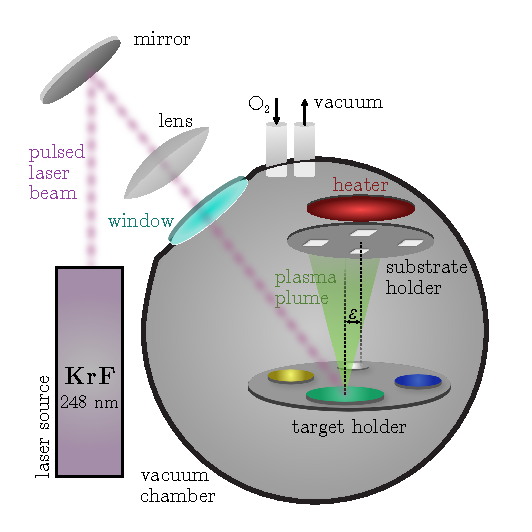
\includegraphics[width=9cm,align=c]{fastImages/PLD.pdf}&
        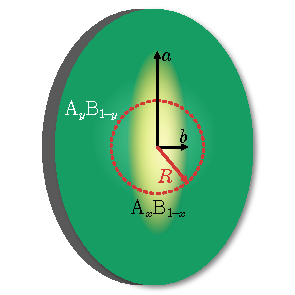
\includegraphics[width=5cm,align=c]{fastImages/target.pdf}  
    \end{tabular}
    \caption{\textbf{(a)} Schematic of a \gls{pld} setup and \textbf{(b)} schematic of an elliptically segmented pellet used as target for \acrshort{DCS}-\gls{pld}.
    $a$ and $b$ are semi-major and semi-minor axis of the ellipse, respectively.
    $R$ denotes the radius of the circular laser spot path on the target surface.
    The composition of the inner and outer segment is \ce{A_xB_{1-x}} and \ce{A_yB_{1-y}}, respectively.}
    \label{Fig:Methods_pld}
\end{figure}

The laser energy density, called fluence $F$, can be calculated by taking the energy per pulse $E$ and the lens position $L$ into account.
For an applied $E=\qty{650}{\milli\joule}$, \qty{75}{\percent} of the energy are absorbed by mirror, lens and entrance window\footnote{
    This was estimated using an energy monitor device and conducted by M.\ Sc.\ J.\ Bredow.}.
This transmittance is assumed to be independent of $E$.
The resulting fluence dependence $F(E,L)=\frac{0.25E}{A(L)}$ is visualized in Fig.\,\ref{Fig:Methods_fluence}, whereby the laser spot size $A$ was measured for some $L$ and fitted by assuming parabolic behavior.

\begin{figure}
    \centering
    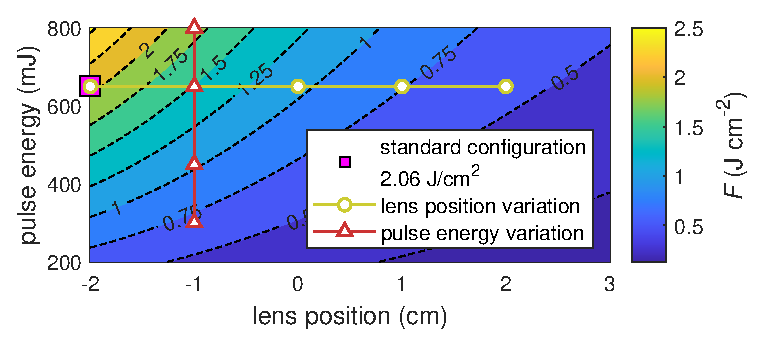
\includegraphics{fluence.eps}
    \caption{Laser energy density depending on the applied pulse energy and lens position. Smaller lens positions yield smaller spot sizes. A value of \qty{-2}{\cm} corresponds to the lens being as close as possible to the laser entrance window in the setup used for this work.
    The default configuration of \qty{650}{\milli\joule} and \qty{-2}{cm} yields typical fluences of about \qty{2}{\J\per\square\cm}.
    The triangles and circles represent the variation of laser fluence in this work, achieved by varying the pulse energy and lens position, respectively.}
    \label{Fig:Methods_fluence}
\end{figure}

\subsection{Plasma Dynamics}
The \gls{pld} procedure can be broken down into three physical processes: (i) energy absorption on the target surface, (ii) formation of a plasma and (iii) condensation on the substrate:
\begin{enumerate}[label=(\roman*)]
    \item After being projected on the surface of the pellet, the radiation penetrates the material only by a fraction of a \unit{\um}.
    Electrons are excited and oscillate in the electromagnetic field of the laser pulse.
    Those electrons collide with bulk atoms of the surface region, which are subsequently heated up and vaporize.
    This process is supported by breaking of chemical bonds due to laser radiation.
    \item A material cloud expands perpendicular to the target surface due to Coulomb repulsion and recoil.
    Absorption of remaining laser radiation results in a plasma plume which is strongly forward directed for low background pressures below \qty{e-4}{\milli\bar}.
    The target is rotating and laterally moving during this process to minimize the deflection of the plasma due to target degradation.
    The kinetic energy of the material in the plasma plume is crucial for the deposition process and can be controlled by background partial pressure and laser energy density on the target.
    \item The plasma plume hits the substrate which can result in resputtering of already deposited material, which condensates together with the plasma, resulting in thermal equilibrium and thus thin film nucleation.
    A large number of adatoms results in many nucleation centers which are responsible for smooth films.
\end{enumerate}
Therefore, \gls{pld} is a non-equilibrium process, making empirical optimization of growth parameters an essential part of thin film manufacturing
    \cite{lorenz2019}.

\subsection{Segmented Target Approach}\label{Sec:Methods_VCCS}
To provide a discrete material library -- a set of different samples with homogeneous composition each --, a segmented target approach as described in \textcite{wenckstern2020} is applied.
Specifically, the \gls{DCS} method utilizes a radially segmented target, i.e.\ a target with distinct regions of different material composition.
By varying the laser spot position on the target, different plasma compositions can be achieved.
Because the target is rotating during \gls{pld}, the material distribution must be in such a way that when the radial position $R$ of the laser on the target changes, the average ablated composition $\chi(R)$ changes.
This can be realized with an elliptical segmentation, i.e.\ a target pellet with overall composition \ce{A_yB_{1-y}}, but containing an inner ellipse with composition \ce{A_xB_{1-x}} (Fig.\,\ref{Fig:Methods_pld}b).
By this means, any homogeneous composition \ce{A_$\chi$B_{1-$\chi$}} with $\chi$ between $x$ and $y$ can be realized with only one target.
$\chi$ is related to the path lengths of the moving laser spot on the inner and outer segment, respectively.
The composition in the plasma can be calculated via \cite{wenckstern2020}:
\begin{equation}\label{Equ:Methods_composition}
    \chi(R) = y-(y-x)\frac{2}{\pi}\arccos\left[\frac{1}{\delta}\sqrt{1-\left(\frac{b}{R}\right)^2}\,\right]\,
\end{equation}
where $\delta$ and $b$ are eccentricity and semi-minor axis of the ellipse, respectively\footnote{
    The eccentricity is defined as $\delta=\sqrt{1-b^2/a^2}$, where $a$ is the length of the semi-major axis.
}.
Small and large $R$ will result in a composition equal to the composition of the inner and outer segment, respectively.
To model the process more accurately one has to take into account that the laser illuminates a finite area rather than a point-like spot.
This is done in~\ref{Sec:Results_Doping}, in particular refer to Fig.\,\ref{Fig:Results_2_yToComposition}. 


\newpage
\sloppy % increases probability of hyphenation
\printbibliography
\end{document}